\title{BT5110 Data Management and Warehousing}

\subtitle{Tutorial 9: Data Warehousing and Dimension Modelling}

\author{Mark Meng Huasong}

\institute[National University of Singapore] % (optional, but mostly needed)
{
	School of Computing\\
	National University of Singapore
}

\titlegraphic{
	
\includegraphics[width=2cm]{nus-logo}
}

\date{1 - 5 Nov, 2021}

\begin{frame}
	\titlepage
	\begin{tcolorbox}
		\begin{center}
			{\scriptsize \textcolor{red}{All the materials within presentation slides are protected by copyrights.\\
					It is forbidden by NUS to upload these materials to the Internet.}}
		\end{center}
	\end{tcolorbox}
\end{frame}

\begin{comment}
\begin{frame}[fragile]{Quick Recap: End of Last Tutorial}
	What we have done in the last week:\\\vspace{5pt}
	(1) Write simple queries with aggregation;\\
	(2) Write nested queries;\\
	(3) Make use of double negation and left outer joining to achieve complex queries. \\\vspace{5pt}
	
\end{frame}
\end{comment}

\section*{Question 1}

\begin{frame}[fragile]{Question 1}
Answer the following questions by quoting the relevant excerpts in the chapter, recalling the relevant examples from the chapter, synthesising an answer in your own words while keeping the main keywords and proposing your own illustrating example or examples.\\\vspace{10pt}
\textbf{Question}: What are the advantages of modeling the data warehouse around business processes rather than around organizational business departments or as a holistic organization wide data warehouse?\\
\vspace{10pt}
\textcolor{blue}{Discussed in Lecture (at around 00:14:30 of the Zoom recording)}
\end{frame}

\begin{frame}[fragile]{Question 1 (Cont.)}
	
\begin{columns}[t]
\column{0.65\textwidth}
\textbf{Solution}: In this document, we only provide the quote from Kimball but the complete answer should also contain Kimball's example, your answer and your own illustrating examples. \\ \vspace{6pt}
From page 30 of \textit{Kimball} Chapter 2: \\ \vspace{6pt}
``By focusing on business processes, rather than on business departments, we can deliver consistent information more economically throughout the organization.''
\column{0.33\textwidth}
\vspace{-15pt}
\begin{figure}
	\frame{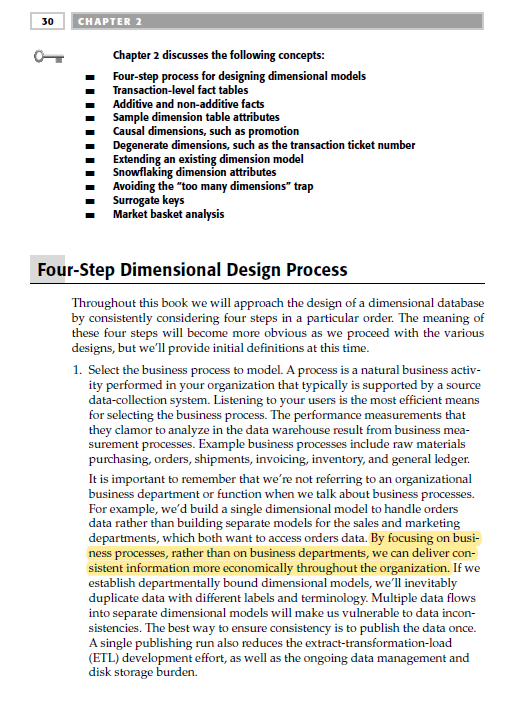
\includegraphics[width=1\textwidth, trim=0 0 0 0, clip]{t9/images/q1.png}}
\end{figure}
\end{columns}
\end{frame}

\begin{frame}[fragile]{Question 1 (Cont.)}
\textbf{Elaboration} (with original text in page 30):\\
\begin{itemize}
	\item We'd build a single dimensional model to handle orders
	data rather than building separate models for the sales and marketing
	departments, which both want to access orders data.
	\item ... establish departmentally bound dimensional models, we’ll inevitably
	duplicate data with different labels and terminology. 
	Multiple data flows
	into separate dimensional models will make us vulnerable to data inconsistencies.
	\item The best way to ensure consistency is to publish the data once.
\end{itemize}
\end{frame}

\section*{Question 2}
\begin{frame}[fragile]{Question 2}
\textbf{Question}: What question entails the choice of the facts?\\\vspace{10pt}

\textcolor{blue}{Discussed in Lecture (at around 00:31:20 of the Zoom recording)}\\\vspace{10pt}

\begin{columns}[t,onlytextwidth]
\column{0.67\textwidth}
\textbf{Solution}: From page 31 of \textit{Kimball} Chapter 2, ``Facts are determined by answering the question, ``What are we measuring?''.''\\ \vspace{10pt}

Facts that clearly belong to a different grain must be in a separate fact
table. Typical facts are numeric additive figures such as quantity ordered or
dollar cost amount.
\column{0.3\textwidth}
\vspace{-15pt}
\begin{figure}
	\frame{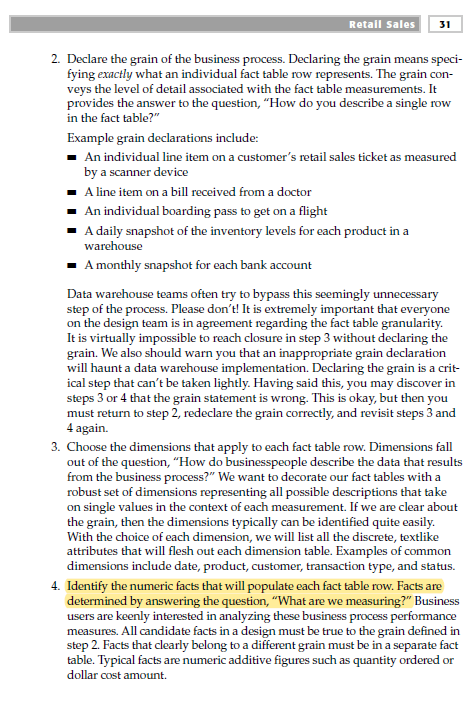
\includegraphics[width=1\textwidth, trim=0 0 0 0, clip]{t9/images/q2.png}}
\end{figure}
\end{columns}
\end{frame}

\section*{Question 3}
\begin{frame}[fragile]{Question 3}
\textbf{Question}: What is an ``additive fact''? Give examples and counter-examples (semi-additive, non-additive).\\\vspace{10pt}
\textbf{Solution}:\\ \vspace{5pt}
\begin{columns}[t,onlytextwidth]
\column{0.68\textwidth}
You may refer to the page 17 to find the definition of various types of facts.\\\vspace{5pt}
More details are given in following slides.
\column{0.3\textwidth}
\begin{figure}
	\vspace{-15pt}
	\frame{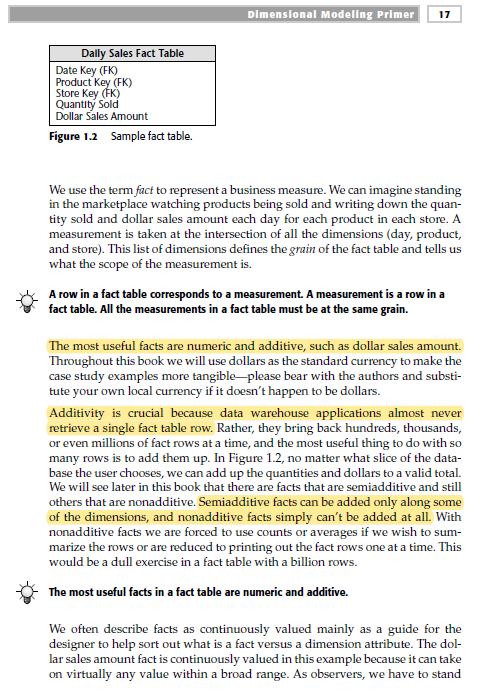
\includegraphics[width=1\textwidth, trim=0 0 0 0, clip]{t9/images/q3.png}}
\end{figure}
\end{columns}
\end{frame}

\begin{frame}[fragile]{Question 3 Cont.}

\textbf{\textit{Additive facts}}: Facts that can be summed up through all dimensions in the fact table.
\\ \vspace{5pt}
\textbf{\textit{Semi-additive facts}}: Facts that can be summed up for some of the dimensions in the fact table, but not others.
\\ \vspace{5pt}
\textbf{\textit{Non-additive facts}}: Facts that cannot be summed up for any of the dimensions present in the fact table.\\\vspace{15pt}
Examples are given in following slides.
\end{frame}

\begin{frame}[fragile]{Question 3 Cont.}
\vspace{-13pt}
\begin{columns}
\column{0.2\textwidth}
\column{0.22\textwidth}
\begin{table}[]
	\begin{tabular}{|c|}
		\hline
		Date          \\ \hline
		Store         \\ \hline
		Product       \\ \hline
		Sales\_Amount \\ \hline
	\end{tabular}
\end{table}
\column{0.22\textwidth}
\begin{table}[]
	\begin{tabular}{|c|}
		\hline
		Date          \\ \hline
		Account         \\ \hline
		Current\_Balance     \\ \hline
		Profit\_Margin \\ \hline
	\end{tabular}
\end{table}
\column{0.2\textwidth}
\end{columns}
\texttt{Sales\_Amount} is an \underline{additive fact}, because you can sum up this fact along any of the three dimensions present in the fact \texttt{table\_date}, \texttt{store}, and \texttt{product}.\\\vspace{3pt}

\texttt{Current\_Balance} and \texttt{Profit\_Margin} are the facts.\\\vspace{3pt}

\texttt{Current\_Balance} is a \underline{semi-additive fact}, as it
makes sense to add them up for all accounts (what's the total current balance for all accounts in the bank?), but it does not make sense to add them up through time (adding up all current balances for a given account for each day of the month does not give us any useful information). \texttt{Profit\_Margin} is a \underline{non-additive fact}, for it does not make sense to add them up for the account level or the day level.\\\vspace{3pt}

Square footage is semi-additive but it is not a fact.
\end{frame}

\section*{Question 4}

\begin{frame}[fragile]{Question 4}
	\textbf{Question}: Should calculated (derived) facts be stored?\\\vspace{10pt}
	
	\textbf{Solution}: From page 37 of \textit{Kimball} Chapter 2, ``Dimensional modelers sometimes question whether a calculated fact should be stored physically in the database. We generally recommend that it be stored physically. In our case study, the gross profit calculation is straight-forward, but storing it \textbf{eliminates	the possibility of user error.}''. \\\vspace{5pt}
	
	Calculated fact eliminates error. They most likely do not consume
	significantly more space. They can therefore be calculated at the time of staging. They could also be defined using views (the fact table becomes a view of background base tables). The views could be materialised.
\end{frame}

\begin{frame}[fragile]{Question 4 (Cont.)}
\begin{columns}[t,onlytextwidth]
	\column{0.68\textwidth}
	\textbf{Elaboration}:\\\vspace{10pt}
	Calculated fact eliminate error. They most likely do not consume significantly more space. They can therefore be calculated at the time of staging.\\\vspace{5pt}
	They could also be defined using views (the fact table becomes a view of background base tables). The views could be materialised.
	More details are given in following slides.
	\column{0.28\textwidth}
	\begin{figure}
		\vspace{-15pt}
		\frame{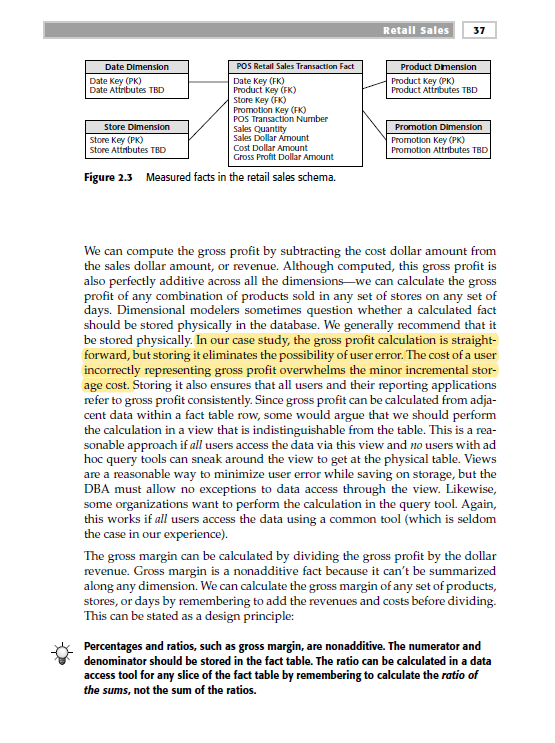
\includegraphics[width=1\textwidth, trim=0 0 0 0, clip]{t9/images/q4.png}}
	\end{figure}
\end{columns}
\end{frame}

\section*{Question 5}

\begin{frame}[fragile]{Question 5}
	\textbf{Question}: What is the ``grain'' or ``granularity''? How to determine the appropriate grain?.\\\vspace{10pt}
	\textcolor{blue}{Discussed in Lecture (at around 00:49:30 of the Zoom recording)}\\\vspace{10pt}
	\textbf{Solution}: From page 31 of \textit{Kimball} Chapter 2, ``Declaring the grain means specifying exactly what an individual fact table row represents.  The grain conveys the level of detail associated with the fact table measurements.''\\\vspace{5pt}
\end{frame}

\begin{frame}[fragile]{Question 5 (Cont.)}
	\textbf{Elaboration}:\\\vspace{5pt}
	``Grain'' or ``granularity'' is the level of details of the data stored in the fact table. The finer the grain, the more rows in the fact table. The coarser the grain the more aggregated the data in the fact table.
	\\\vspace{5pt}
	\begin{columns}[t,onlytextwidth]
		\column{0.69\textwidth}
		The grain is determined by specifying exactly what an individual fact table row represents. It answers the question ``How do you describe a single row in the fact table?'' A grain declaration could be:\\
		\begin{itemize}
			\item An individual line item on a customer's retail sales ticket as measured by a scanner device;
			\item A line item on a bill received from a doctor;
			\item A daily snapshot of the inventory levels for each product in a warehouse;
			\item A monthly snapshot for each bank account.
		\end{itemize}
		
		\column{0.29\textwidth}
		\begin{figure}
			\vspace{-15pt}
			\frame{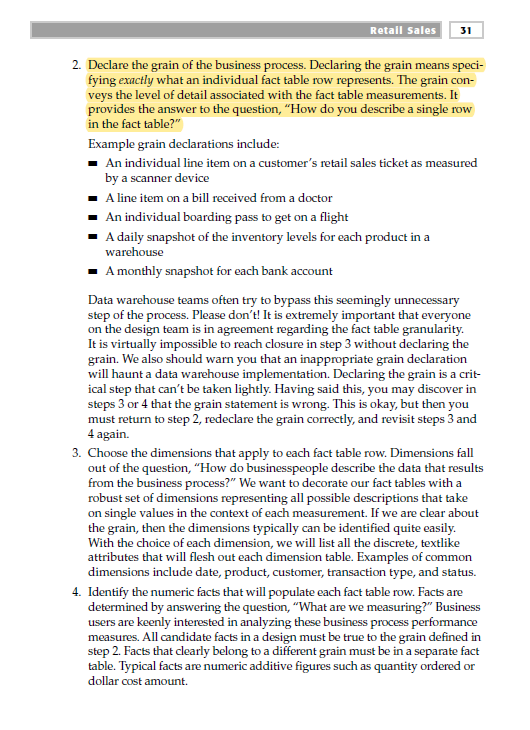
\includegraphics[width=1\textwidth, trim=0 0 0 0, clip]{t9/images/q5.png}}
		\end{figure}
	\end{columns}
\end{frame}
\section*{Question 6}

\begin{frame}[fragile]{Question 6}
	\textbf{Question}: Should there be null values in the fact table? Why?
	\\\vspace{10pt}
	\textbf{Solution}: 
	\\\vspace{5pt}
	\begin{columns}[t,onlytextwidth]
	\column{0.65\textwidth}
	From page 49 of \textit{Kimball} Chapter 2:\\\vspace{5pt}
	``You \textcolor{red}{\textbf{must}} avoid null keys in the fact table. A proper design includes a row in the corresponding dimension table to identify that the dimension is not applicable to the measurement.''
	\column{0.29\textwidth}
	\begin{figure}
		\vspace{-15pt}
		\frame{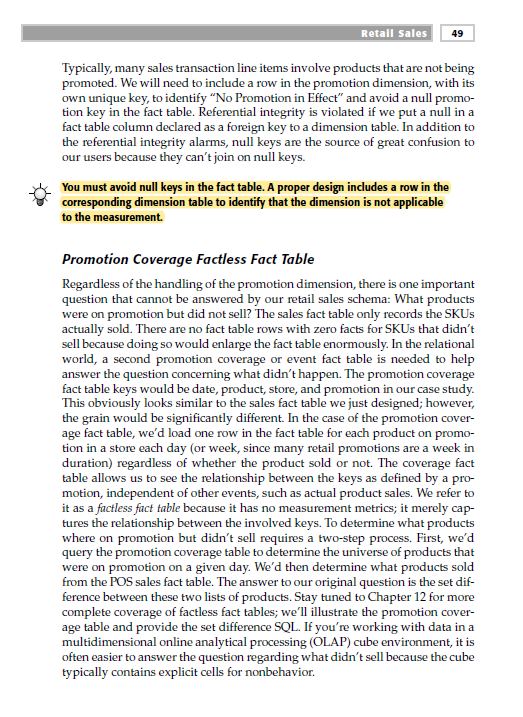
\includegraphics[width=1\textwidth, trim=0 0 0 0, clip]{t9/images/q6.png}}
	\end{figure}
\end{columns}	
\end{frame}

\begin{frame}[fragile]{Question 6 (Cont.)}
	The fact table is composed of attributes corresponding to surrogate keys referencing dimensions and to facts corresponding to measurements. The former cannot be null. \\\vspace{5pt}
	Special situations such as that of a description not being available can be handled by referencing to an explicit description of the situation in the dimension table. \\\vspace{5pt} 
	Measurements, however, can be null, if their value is unknown or does not exist. This is however to be handled with care when asking queries, given the not always appropriate handling of null values in SQL.
\end{frame}
\section*{Question 7}

\begin{frame}[fragile]{Question 7}
	\textbf{Question}: What questions entails the choice of the dimensions?\\\vspace{10pt}
	
	\textbf{Solution}: From page 31 of \textit{Kimball} Chapter 2,
	``Dimensions fall out of the question, ``How do business people describe the data that results from the business process?''.''\\\vspace{5pt}
	\begin{columns}[t,onlytextwidth]
		\column{0.72\textwidth}
		We want to decorate our fact tables with a robust set of dimensions representing all possible descriptions that take on single values in the context of each measurement.%\\\vspace{5pt}
		If we are clear about the grain, then the dimensions typically can be identified quite easily. With the choice of each dimension, we will list all the discrete, textlike attributes that will flesh out each dimension table.%\\\vspace{5pt}
		Examples of common dimensions include date, product, customer, transaction type, and status.
		 
		\column{0.26\textwidth}
		\begin{figure}
			\vspace{-15pt}
			\frame{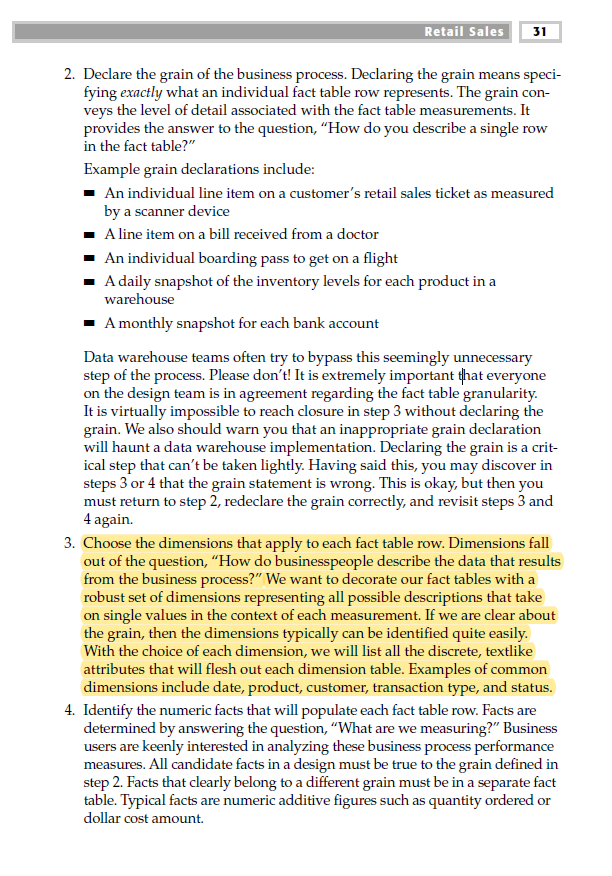
\includegraphics[width=1\textwidth, trim=0 0 0 0, clip]{t9/images/q7.png}}
		\end{figure}
	\end{columns}
\end{frame}

\section*{Question 8}

\begin{frame}[fragile]{Question 8}
	\textbf{Question}: What is the role of descriptive attributes in dimensions?\\\vspace{10pt}
	
	\textbf{Solution}: \\\vspace{5pt}
	\begin{columns}[t,onlytextwidth]
	\column{0.67\textwidth}They are entry point for queries. There can be many and should be as many as needed.\\\vspace{5pt}	
	From page 21 of \textit{Kimball} Chapter 1, ``the fact table consisting of numeric measurements is joined to a set of dimension tables filled with descriptive attributes.''
	\column{0.28\textwidth}
	\begin{figure}
		\vspace{-15pt}
		\frame{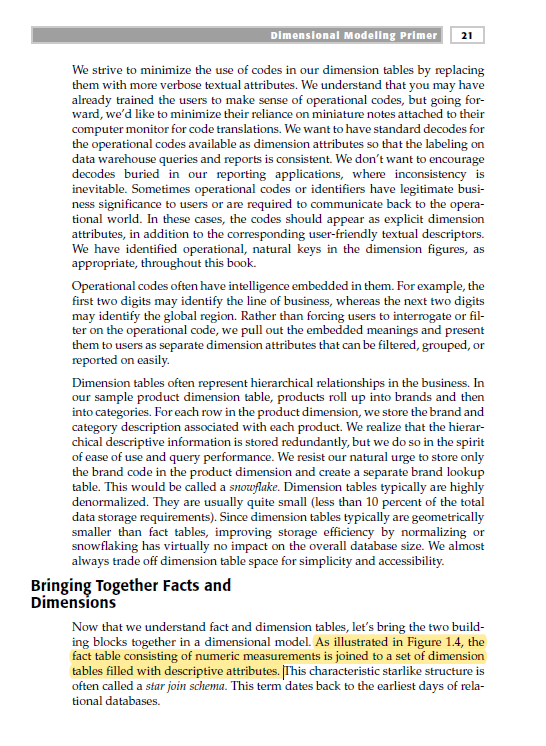
\includegraphics[width=1\textwidth, trim=0 0 0 0, clip]{t9/images/q8.png}}
	\end{figure}
\end{columns}
\end{frame}

\begin{frame}[fragile]{Question 8 (Cont.)}
	Each attribute is a rich source for constraining and constructing row headers. If we want to drill down, we can drag virtually any other attribute and we automatically drill down to this next level of detail.\\\vspace{5pt}	
	Drilling down is nothing more than adding row headers from the dimension tables. Drilling up is removing row headers.\\\vspace{5pt}	
	A robust and complete set of dimension attributes translates into user capabilities for robust and complete analysis.
\end{frame}

\section*{Question 9}

\begin{frame}[fragile]{Question 9}
	\textbf{Question}: Should there be null values in the dimension tables? Why? \\\vspace{10pt}
	
	\textbf{Solution}: Null values \textcolor{blue}{\textbf{should}} be \textbf{avoided} in the dimension tables. Attributes of the dimension tables are used for aggregation. Group do not behave smoothly with null value
\end{frame}

\section*{Question 10}

\begin{frame}[fragile]{Question 10}
	\textbf{Question}: What is Kimball's argument in favour of surrogate keys?\\\vspace{10pt}
	
	\textbf{Solution}: \\\vspace{5pt}
	\begin{columns}[t,onlytextwidth]
		\column{0.67\textwidth}From page 59 of \textit{Kimball} Chapter 2: \\\vspace{5pt}
		``In general, we want to avoid embedding intelligence in the data warehouse keys because any assumptions that we make eventually may be invalidated.''
		\column{0.28\textwidth}
		\begin{figure}
			\vspace{-15pt}
			\frame{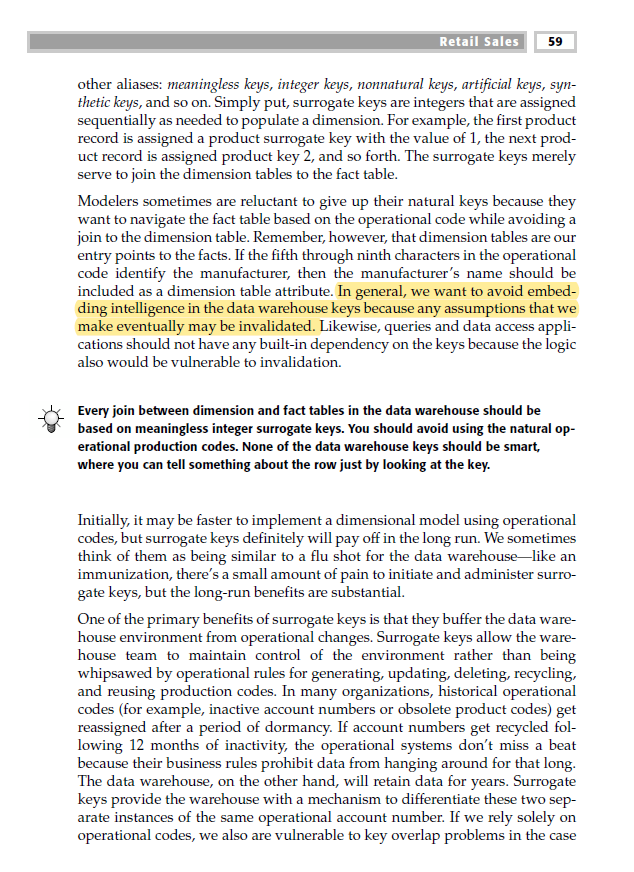
\includegraphics[width=1\textwidth, trim=0 0 0 0, clip]{t9/images/q10.png}}
		\end{figure}
	\end{columns}
\end{frame}

\begin{frame}[fragile]{Question 10 (Cont.)}
	Surrogate keys = ``fake'' keys, such as an incremental ID.\\\vspace{5pt}
	Surrogate keys provide the warehouse with a mechanism to differentiate two separate instances of the same operational number that wouldn't be possible if the operational number was used directly.\\\vspace{5pt}
	If we rely solely on operational codes, we also are vulnerable to key overlap problems in the case of an acquisition or consolidation of data.
	Performance advantages: Can be a small integer.\\\vspace{5pt}
	The surrogate keys should merely serve to join the dimension tables to the fact table.
\end{frame}

\section*{Question 11}

\begin{frame}[fragile]{Question 11}
	\textbf{Question}: What can be said about the relationship between grain and dimensions? \\\vspace{10pt}	
	\textbf{Solution}: The finer the grain the more dimensions.\\\vspace{5pt}
	The grain of the dimensional model is the finest level of detail that is implied when the fact and dimension tables are joined.\\\vspace{5pt}
	For example, the granularity of a dimensional model that consists of the dimensions Date, Store, and Product is ``product sold in store by day''.\\\vspace{5pt}
	For example, a dimension such as Date (with Year and Quarter hierarchies) has a granularity at the quarter level but does not have information for individual days or months.	
\end{frame}

\begin{frame}[fragile]{}
	\centering  
	For any further question, please feel free to email me:\vspace{10pt}
	
	huasong.meng@u.nus.edu \vspace{20pt}
	
	\begin{tcolorbox}
		\begin{center}
			\textcolor{red}{Cases in the extra practice are contributed by our students.\\\vspace{5pt}Copyright 2021 Mark H. Meng. All rights reserved.}
		\end{center}
	\end{tcolorbox}
\end{frame}
